\begin{figure*}[t]
\centering
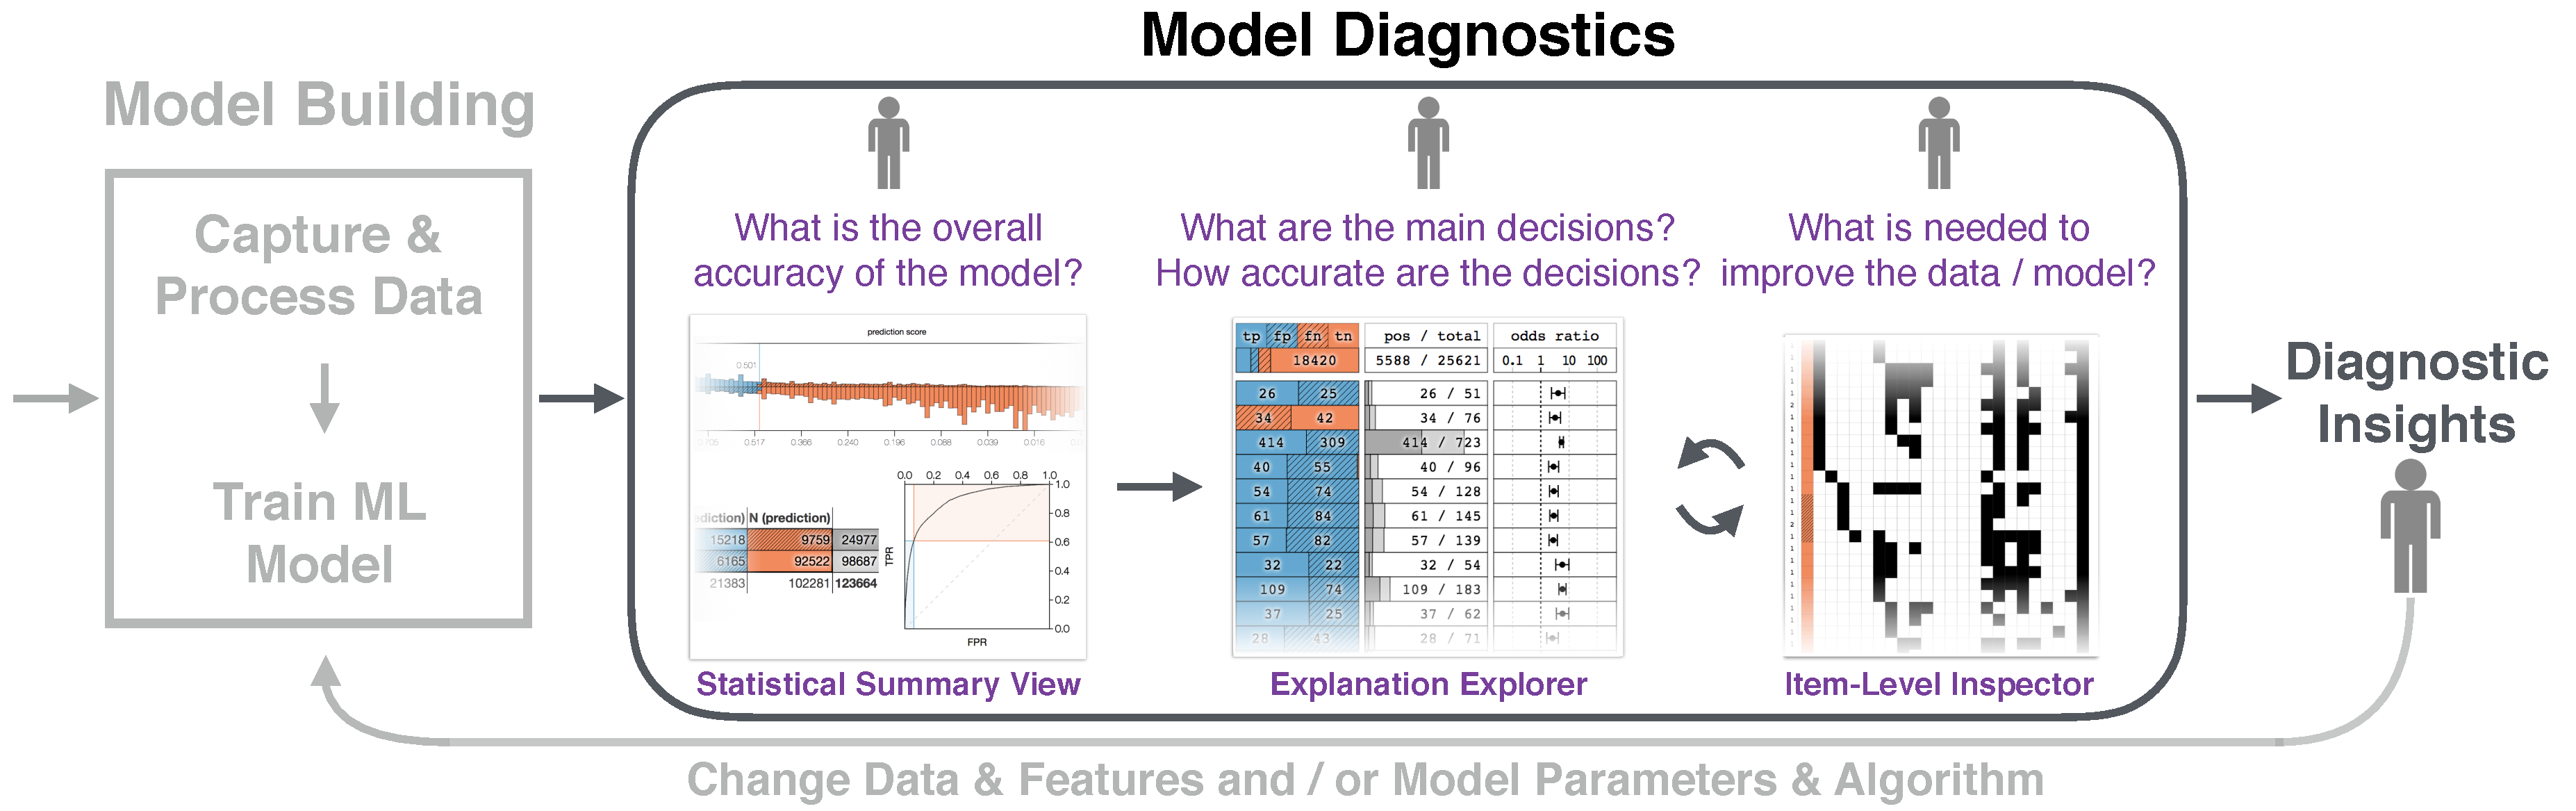
\includegraphics[width=\textwidth]{explainer/workflow5}
\vspace{-3mm}
\caption{
Our proposed \textbf{Model Diagnostics} workflow extends the conventional \textit{Model Building} workflow in machine learning for enabling domain experts to reason about the semantic validity of the decisions made by any model through multiple linked visualizations of statistical performance summaries, explanations, and item-level distribution of features. By iterating through explanation-level summaries and item-level details, experts are able to generate diagnostic insights about the quality of both the data and the model. This ultimately helps to improve data acquisition and model generation processes belonging to the original workflow.
}
\vspace{-5mm}
\label{figs:workflow}
\end{figure*}

% An explanation comprises of a set of features that need to be removed to change the label for a given item. 